%%%%%%%%%%%%%%%%%%%%%%%%%%%%%%%%%%%%%%%%%%%%%%%%%%%%%%%%%%%%%%%%%%%%%%%%
%    INSTITUTE OF PHYSICS PUBLISHING                                   %
%                                                                      %
%   `Preparing an article for publication in an Institute of Physics   %
%    Publishing journal using LaTeX'                                   %
%                                                                      %
%    LaTeX source code `ioplau2e.tex' used to generate `author         %
%    guidelines', the documentation explaining and demonstrating use   %
%    of the Institute of Physics Publishing LaTeX preprint files       %
%    `iopart.cls, iopart12.clo and iopart10.clo'.                      %
%                                                                      %
%    `ioplau2e.tex' itself uses LaTeX with `iopart.cls'                %
%                                                                      %
%%%%%%%%%%%%%%%%%%%%%%%%%%%%%%%%%%
%
%
% First we have a character check
%
% ! exclamation mark    " double quote  
% # hash                ` opening quote (grave)
% & ampersand           ' closing quote (acute)
% $ dollar              % percent       
% ( open parenthesis    ) close paren.  
% - hyphen              = equals sign
% | vertical bar        ~ tilde         
% @ at sign             _ underscore
% { open curly brace    } close curly   
% [ open square         ] close square bracket
% + plus sign           ; semi-colon    
% * asterisk            : colon
% < open angle bracket  > close angle   
% , comma               . full stop
% ? question mark       / forward slash 
% \ backslash           ^ circumflex
%
% ABCDEFGHIJKLMNOPQRSTUVWXYZ 
% abcdefghijklmnopqrstuvwxyz 
% 1234567890
%
%%%%%%%%%%%%%%%%%%%%%%%%%%%%%%%%%%%%%%%%%%%%%%%%%%%%%%%%%%%%%%%%%%%
%
\documentclass[12pt]{iopart}
\usepackage{graphicx,epstopdf}
\usepackage{caption}
\usepackage{subcaption}
\graphicspath{ {./figs/} }
%Uncomment next line if AMS fonts required
%\usepackage{iopams}
\begin{document}

\title[Modeling a Neural Co-Processor]
{Towards a Neural Co-Processor Which Restores Movement After Stroke: Modeling a Proof-of-Concept}

\author{Matthew J Bryan$^{1}$, Linxing Preston Jiang$^{1}$, Rajesh P N Rao$^{1}$}

\address{$^{1}$ Neural Systems Laboratory, Department of Computer
Science and Engineering, University of Washington, Box 352350,
Seattle, WA 98105, USA}

\ead{matthew.bryan@dell.com}
\vspace{10pt}
\begin{indented}
\item[]September 2021
\end{indented}

\begin{abstract}
\textit{Objective} Brain co-processors\cite{rao.coproc} are devices which use artificial
intelligence (AI) for closed-loop neurostimulation, to shape neural activity and to bridge
injured neural circuits for targeted repair and rehabilitation. The co-processor framework
offers a flexible approach to learning closed-loop stimulation policies that optimize for
(a) specific regimes of neural activity, or (b) external task performance.
For example, it may seek to learn to stimulate the motor cortex of a stroke patient,
conditioning the stimulation on upstream visual information, aiding the patient's
attempt to grasp an object. Through the use of artificial neural
networks (ANNs) and deep learning, the co-processor co-adapts with the
neural circuit, allowing it to seek optimal stimulation policies, and adapt them
as the neural circuit changes. The results presented here demonstrate a
neural co-processor for the first time, through the use of a simulation. We
explore some of the core algorithms that may allow co-processors to successfully
learn and to adapt to non-stationarity in both the brain and sensors.
\textit{Approach} We provide the first proof-of-concept of a neural co-processor that
leverages deep learning, through the use of a simulated neural circuit.
That circuit performs reach-to-grasp task, based on visual input, and is designed to
closely resemble a similar circuit in a primate brain \cite{michaels.mrnn}. We simulate
a variety of lesions by altering the model, and then demonstrate our co-processor's ability
to restore lost function through ``stimulation'' of that model. We further test the
ability of our co-processor to adapt its stimulation as the simulated brain undergoes changes.
\textit{Main results} Our simulated co-processor successfully co-adapts with the neural
circuit to accomplish the external reaching task. The co-processor framework
demonstrated here adapts to a variety of lesion types, and to ongoing changes in the
simulated brain.
\textit{Significance} The proof-of-concept here outlines a co-processor model, as well
as our approach to training it, leading to insights on how such a model may be
developed for \textit{in vivo} use. We believe this co-processor design will allow for
learning complex stimulation policies that help restore function to a stroke victim.
\end{abstract}

\vspace{2pc}
\noindent{\it Keywords}: brain-computer interface, neural co-processor, ai, machine learning, stimulation
%
% Uncomment for Submitted to journal title message
%\submitto{\JPA}
%
% Uncomment if a separate title page is required
\maketitle
% 
% For two-column output uncomment the next line and choose [10pt] rather than [12pt] in the \documentclass declaration
%\ioptwocol
%



\section{Introduction}
Aided in part by application of advanced AI techniques, brain-computer interfaces (BCIs) have made
advancements over the last several decads, allowing for decoded brain signals to be used for
control of a wide variety of virtual and physical prostheses \cite{rao.bcibook, wolpaw.bcibook,
moritz.neuro, lebedev.bmi}. Separately: advances in stimulation techniques and modeling have allowed
us to probe neural circuit dynamics (e.g. \cite{walker.inception}) and learn to better drive neural
circuits towards target dynamics, by encoding and delivering information through
stimulation \cite{niparko.cochlear, weiland.retinal, tomlinson.propr, tabot.tact, tyler.tact,
dadarlat.tact, sharlene.tact, cronin.tact}.
Recently, there has been increasing interest in building on these advances to combine decoding
and encoding in a single system, for closed-loop stimulation of a neural circuit. Bi-directional
BCIs (BBCIs) allow stimulation to be conditioned by decoded brain activity as well as external
sensor data (e.g. camera), which can allow for the application of real-time, fine-grained control of
neural circuits and prosthetic devices, e.g. Nicolelis et al. \cite{nicolelis.bmbi}. These may lead,
for example, to neuro-prostheses that are capable of restoring movement which was lost due to
traumatic brain injury (TBI), to a degree not previously possible.

Motivated by that progress, we demonstrate here a flexible framework for combining encoding
and decoding, which we term ``neural co-processors'' \cite{rao.coproc}. Neural co-processors leverage
AI and deep learning to identify optimal, closed-loop stimulation patterns. The approach is flexible
enough to optimize not only for particular neural activities, but also for tasks external to the
subject. For example, they may be able to aid a stroke victim by finding a stimulation pattern of
the motor cortex which helps restore lost limb function. Likewise, the framework generalizes enough
to condition stimulation on both brain activity, and external sensors, e.g. cameras or LIDAR, in
order to incorporate feedback for realtime control.

Additionally, the co-processor framework allows a neuro-prosthesis to actively adapt to
a neural circuit as it changes with time. This framework is capable of co-adapting with
the circuit, i.e. brain, by updating its stimulation regime, while at the same time the
brain is updating its response to the stimulation, and changing due to natural plasticity,
aging, etc. This allows the co-processor to continually optimize for the intended cost
function, despite the signficant non-stationarity of the target circuit.

Here we provide a proof-of-concept in simulation for a co-processor that restores
movement to a limb, after a subject has suffered a stroke affecting its ability to
use that limb. It combines:
\begin{itemize}
	\item A stimulation model, which models the relationship between decoded brain activity,
	      stimulation, and task performance.
	\item An AI agent which determines the stimulation to apply in a closed-loop fashion, in real time.
\end{itemize}

Significant advances have been made in modeling the effects of electrical stimulation
of the brain, some of which can be leveraged for our co-processor design, as we outline
below. Researchers have explored how information can be biomimetically or
artificially encoded and delivered via stimulation to neuronal networks in the brain and
other regions of the nervous system for auditory \cite{niparko.cochlear}, visual \cite{weiland.retinal},
proprioceptive \cite{tomlinson.propr}, and tactile
\cite{tabot.tact, tyler.tact, dadarlat.tact, sharlene.tact, cronin.tact} perception.
Advancements have also been made in modeling the effects of stimulation over large scale, multi-region
networks, and across time \cite{shanechi.stimmodel}. Some have additionally designed models which
can adapt to ongoing changes in the brain, including changes due to the stimulation itself
\cite{tafazoli.acls}. In our proof-of-concept outlined below, we will use a stimulation
model, not unlike those cited here, which seeks to account for both network dynamics
and non-stationarity. In addition to training the model to have a strong ability to predict
the effect of stimulation, we additionally train it to be useful for then learning an
optimal stimulation policy, which is a property somewhat distinct from predictive
power alone.

Advances have also been made in both open- and closed-loop stimulation for
treating a variety of disorders. Open loop stimulation has been effective in
treating Parkinson's Disease \cite{benabid.parkinsons}, as well as various
psychiatric disorders \cite{holtzheimer.psy, kisely.psy, fraint.psy}.
More directly related to this paper, we see in Khanna et al. \cite{khanna.openloop},
the use of open loop stimulation in restoring dexterity after a lesion
occurs affecting a primate's motor cortex. The authors demonstrate that
the use of low-frequency alternating current, applied epidurally and set to
certain phases, can improve grasp performance.

While open loop stimulation techniques have yielded clinically useful results,
their results in many domains have been mixed, such as use in visual
prostheses \cite{bosking.visual}, and use in invoking somatosensory feedback
\cite{cronin.tact}. Likely this is due to the stimulation not being conditioned
on the ongoing dynamics of the circuit being stimulated. Moment-to-moment and
throughout the day, the circuit will respond differently to the same stimulus,
as a result of differing inputs and ongoing activity. Stimulation
therefore needs to be proactively adapted in response. This need is even
greater over longer time scales as the effects of plasticity and ageing change
the connectivity of the brain.

Closed-loop stimulation conditions stimulation on observations of brain activity,
possibly allowing it to shape the neural activity more precisely, and to adapt to changes
in the circuit over time. This opens the door to real-time, targeted control of the neural
circuit. It has been used to aid in learning new memories after some impairment
\cite{berger.closedloop, kahana.biomarker}, to replay visually-invoked
activations \cite{tafazoli.acls}, and for optogenetic control of
a thalamocortical circuit \cite{bolus.opto}, among others.

Something that remains unclear is how to leverage closed-loop control for real-time
co-adaption with the brain to accomplish an external task. ``Co-adaption'' here refers
to the ability of a neuro-prosthesis to adapt its stimulation regime to the ongoing
changes in the circuit it is stimulating, and to adapt with that circuit to accomplish
the external task, such as grasping. The neural co-processor we present here provides one
potential model for accomplishing that. Through the use of deep learning, the
co-processor model we present co-adapts an AI agent, which governs the
stimulation, with both a stimulation model, and the neural circuit being stimulated.

For a neurologically complex task such as grasping, we cannot identify
\textit{a priori} a real time controller of the neural circuit. That is
due in large part to the variability of circuits from subject-to-subject,
as well as variations in the placement of sensors and stimulators in the
brain. The only plausible path to such a real time controller is to parameterize
it in a subject- and time-specific way. Our model seeks to accomplish that using
deep learning, together with a data-efficient approach to training.

Before attempting \textit{in vivo} experiments using such a model, we first demonstrate
here a number of crucial design elements of it, through the use of a simulated
grasping circuit, presented previously by Michaels et al. \cite{michaels.mrnn}. We
explore:
\begin{itemize}
	\item The properties of the artificial neural networks (ANNs) that are needed to
	      successfully adapt to the long-running dynamics of a stimulated neural circuit,
	      as well as to adapt to that circuit's ongoing changes.
	\item Data-efficient methods for training these models, to better ensure we
	      can train them with a biologically-realistic amount of data.
	\item How we must train our stimulation model to make it effective in later
	      training our stimulation agent.
\end{itemize}

\section{Method}

\begin{figure}
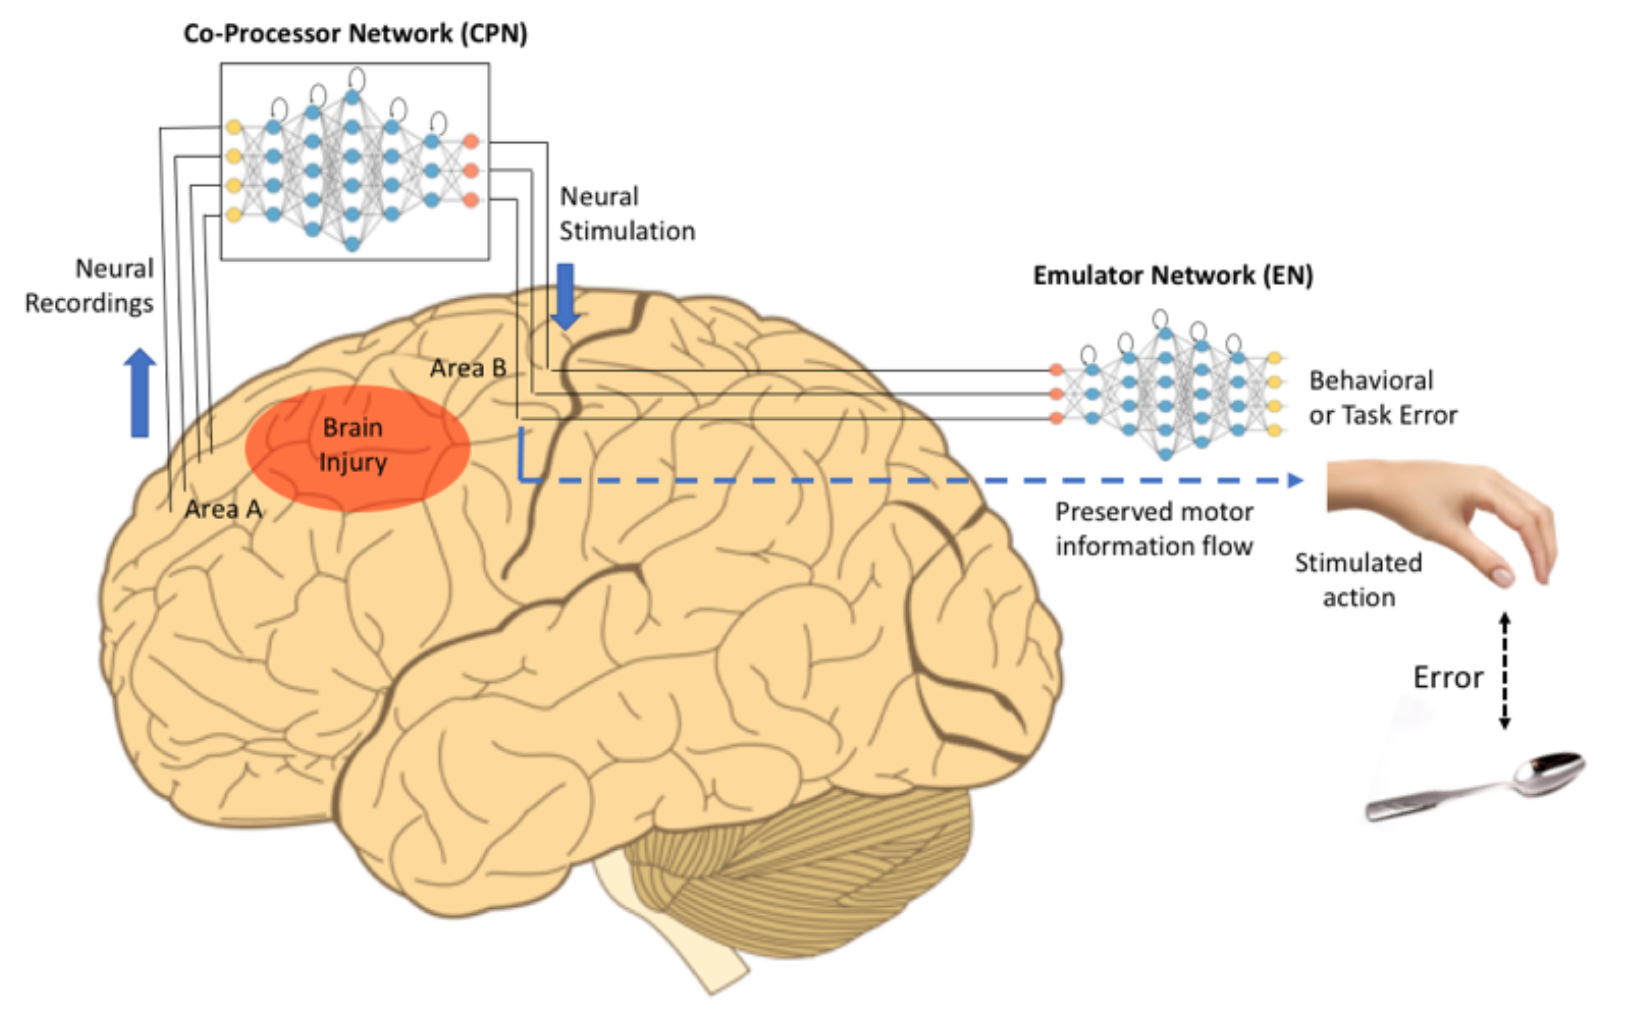
\includegraphics[width=\textwidth]{weill_arch.png}
\caption{Using a co-processor to drive external task performance after a traumatic brain injury}
\centering
\label{fig:weill}
\end{figure}

\subsection{Architecture Overview}
First, we present the architecture of our co-processor design. This design aims to solve two
fundamental challenges in using neural stimulation to improve external task performance.
First, neural networks exhibit long-running and nonlinear dependencies, necessitating
the need for a stimulation agent to account for far-distant effects of the stimulation it
applies. Second, with neurologically complex tasks, such as grasping, the mapping between
neural activity as-measured and the external task cannot be determined \textit{a priori}.
As a result, the co-processor must somehow learn what stimulation is appropriate for
aiding the user in the external task they are attempting to perform.

Our co-processor attempts to solve these with a pair of artificial neural networks:
\begin{itemize}
	\item A stimulation and neural dynamics model, known as an ``Emulator Network'' (EN). It models the relationship
	      between the stimulation, neural dynamics, and external task. It's purpose is for training the second network.
	\item A stimulation agent, known as the ``co-processor network'' (CPN), which maps neural activity, and possibly
	      data from external sensors, to stimulation parameters.
\end{itemize}

We co-train the EN and CPN, with the goal of training a CPN whose output stimulation parameters
improve task performance. By continually training both, they adapt to the brain as it changes,
effectively allowing for brain-stimulator co-adaptation. The EN is a tool for training the CPN,
giving us a way to back-propagate task error to the CPN. It outputs task-relevant
metrics - a prediction of muscle velocities in our case - given measurements of neural
activity, and the stimulation parameters output from the CPN. If the EN is trained in a
particular way, and to a sufficient level of precision, it can be used as a function
approximator relating stimulation and a task, and do so in a way that allows us to train
the CPN with it. When training the CPN, we in-effect treat the EN's output as the true
task performance, or a related metric, and then backpropagate the loss defined in terms
of that metric in order to train the CPN. See Fig. \ref{fig:weill}. We will illustrate the details
of the training algorithm below.

In our present demonstration, the EN is constituted as a single layer, fully connected,
long short-term memory (LSTM) recurrent neural network (RNN), with hyperbolic tangent ($tanh$)
activations, and a linear readout. The general notion of a co-processor does
not require this precise architecture, but for our example, we found that the LSTM
approach allows the network to continuously adapt to long-running dependencies in
the simulated neural dynamics, far better than a vanilla RNN. The CPN is constituted
as an almost identical network, though with a different dimensionality, as we explain
below. There is no strict requirement for the EN and CPN to be so similar, but we
found this simple architecture to work well in our example.

Note that the EN effectively constitutes a stimulation model. Its design is
somewhat motivated by the common linear time-invariant state space model of
stimulation, as in e.g. Yang et al. \cite{shanechi.stimmodel}, which is a helpfully
simple (linear) approach. That approach seeks to model neural network dynamics in
terms of a stationary linear model, which, due in part to its simplicity and the
number of techniques developed for it, lends itself to useful interpretations and
analyses of those neural dynamics.

There are some key differences between that approach and the EN architecture we
present here. Our EN's purpose is simply to train the CPN, so we pick an
architecture we find to be best suited to that job. First, our EN architecture
is not linear, through the use of a $tanh$ activation function. That allows us
to escape some of the limits in representational power of linear models, though
we didn't deeply test a strictly linear approach.
Second, LSTM cells are designed to better capture long-running network
dynamics, and in our case we found that they were crucial for that reason:
when using vanilla RNN cells, our co-processor wasn't able to train well.
Compare that to the simpler cells commonly used in vanilla RNNs, which
yield functionally the same approach as the linear state space model, less
the use of a nonlinear activation function.

\subsection{Simulation Overview}
We demonstrate our approach here using a simulated grasping circuit.
A detailed simulation such as this allows us to explore some of the critical
architectural details and training algorithms for a co-processor of this type.
By first doing such exploration in simulation, we are able to rapidly and
cheaply iterate on our design, prior to any \textit{in vivo} experiments.
In order for the simulation to be admissible, we need to ensure it has some
properties that allow it to strongly indicate if our design is improving in
a direction that will later allow for real deployments. Otherwise, our
design may be adapting to the pecularities of the simulation, without
becoming more useful for the real world.

An example of such a simulation approach is Bernal et al. \cite{bernal.sim}. In this work, the
authors use a simulated spiking neural network to train a stimulation agent, much
like the work we present here. Their stimulation agent sought to restore the network's
control of a simulated arm, to reach a target, after a simulated lesion was applied.
As they point out, we have a limited ability to probe a neural circuit \textit{in vivo}
in order to perform learning. As a result, we first need to design our approach through
the use of an admissible simulation. The authors in this case simulated lesions by
effectively removing parts of their simulated network, or by cutting connections between
parts of the network. Likewise here, we use an established design for an artificial
neural circuit which performs a grasping task, whose architecture and training methods
were designed specifically to result in naturalistic dynamics.

The simulated circuit, from Michaels et al. \cite{michaels.mrnn}, was trained
to resemble the grasping circuits of monkey subjects engaged in a delayed reach-to-grasp task.
Its design draws on a body of literature focused on architectures and training methods for RNNs which
seek to create artificial neural circuits that have activation dynamics similar to natural circuits,
including delayed grasping tasks \cite{susillo.mrnn}. The Michaels circuit consists of a
``modular'' vanilla RNN (mRNN), and a linear readout layer. Each ``module'' consists of 100 vanilla
RNN neurons, with a non-linearity applied on the outputs. The modules are internally fully connected,
and are connected to each other sparsely (10\% connectivity). The inputs are visual features
intended to capture the view the monkeys had during the task, specifically VGGNet features from 3D
renderings of the same objects which the monkeys grasped. The outputs are muscle length
velocities for the should, arm, and hand of the monkey during the trial. The natural
velocities were captured with a motion capturing glove, and the artificial neural network
was trained to recapitulate those grasping motions. Data and trained models from this work
were supplied to us by the lead author Jonathan Michaels, for the purpose of our present
simulation. We re-implemented his models' logic in PyTorch, and loaded his trained parameters
into it, for one of his subjects, arbitrarily chosen. See Fig. \ref{fig:michaels}.

\begin{figure}
	\centering
	\begin{subfigure}[c]{0.69\textwidth}
		\centering
		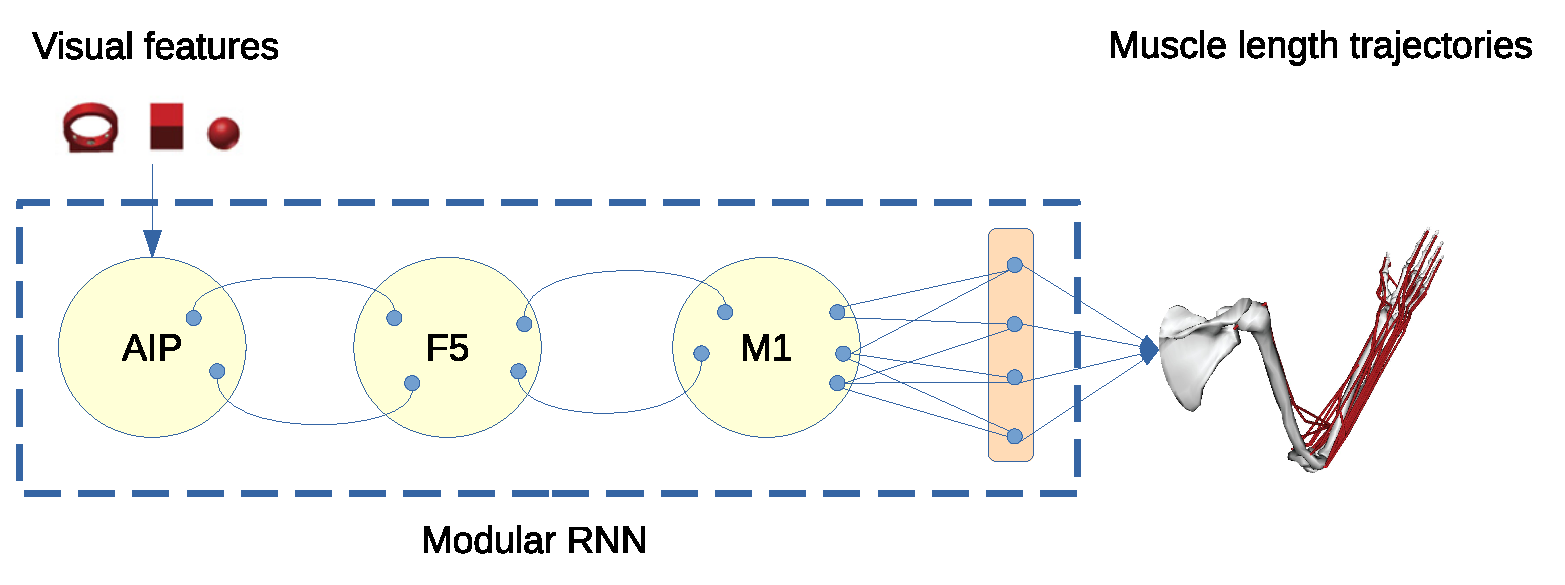
\includegraphics[width=\textwidth]{michaels.eps}
		\caption{Michaels Modular RNN (mRNN), a simulated grasping circuit. The emergent dynamics of the
		three modules correspond well to natural neural activity measured from primate AIP, F5, M1 regions,
		respectively, from the same task. Visual (VGGNet) features forward propagate through the
		network, conditioning the grasp for the object of the particular size, shape, and location.}
	\end{subfigure}
	\hfill
	\begin{subfigure}[c]{0.30\textwidth}
		\centering
		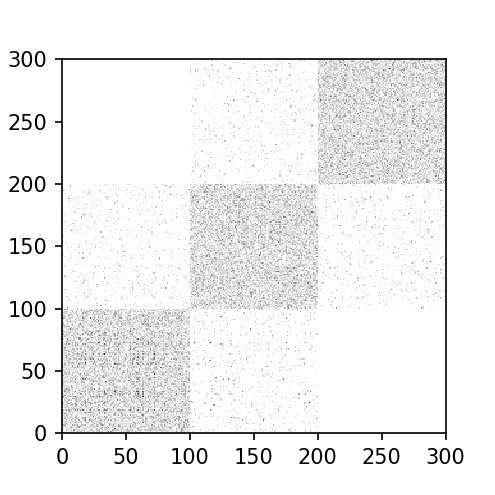
\includegraphics[width=\textwidth]{mRNN_J.png}
		\caption{Connectivity matrix $J$. Note the within-module connections
		(on the diagonal) are fully connected, and connections to adjacent
		modules are sparse $10\%$.}
	\end{subfigure}
	\hfill
\caption{Architecture of the Michaels mRNN}
\label{fig:michaels}
\end{figure}

The design of the circuit is intended to resemble a vision-to-grasp pipeline, essentially
representing the visual processing needed to reach the hand to the appropriate position for
the grasp, and to form the hand properly for grasping the particular shape of object. The
emergent dynamics of the artificial network's ``modules'', once trained, correspond roughly
to the AIP, F5, and M1 portions of the monkey subjects' brains. `Correspond' here, notably,
refers to the fact that the activity of the module receiving the visual inputs resembles
the AIP activity of the monkey subject from the same trials. Likewise, the second and
third modules resemble the natural activity from the monkey's F5 and M1 regions, respectively.
The emergent network dynamics show a number of other correspondences to the monkeys' natural
brain activity as well, as detailed in the paper.

Importantly, the simulated circuit's activity shows a relatively clear separation of the
object shapes. That is - the visual information input to the network that differentiates
one trial from another is leveraged by the circuit to properly condition
the hand shape trajectory for grasping the object of that trial's particular shape, size, and
location. The visual information forward-propagates through the network, through successive
processing steps, where it is eventually leveraged to recapitulate the grasp appropriate
for the object represented by the input visual features. It follows, then, that the classes
are separable in some way by observing the distinct ways that the mRNN is activated by the
classes' corresponding visual inputs. As we will note below: in the absense of this
visual information forward propagating, the circuit can at-best learn a loss-minimizing grasp,
stereotyped across all object sizes and shapes. Such a grasp bears some resemblance to all
grasps the given monkey performed, due to all trials being a reach-to-grasp preceded by a
waiting period, but performance suffers drastically.

\subsubsection{Simulated lesions cause real world failure modes}
Simulating a brain lesion in terms of this artificial network results in error
modes that resemble a natural lesion of certain regions of a primate brain. For example, if we
alter the network by zeroing the outputs of some of the first (input, or AIP) module's neurons,
the reaching motion generally succeeds, but the finger muscle velocities show a high degree
of error - effectively implying that the subject can somewhat reach to grasp, but cannot form a
grasp appropriate for the object. That suggests that losing a portion of the cortical
machinery needed to translate or forward-propagate object shape information
to movement-related cortex can result in a reduced ability to form the hand properly for
the grasp, though positioning of the hand may still roughly succeed. Muscle spasticity of
the hand is also a common symptom of certain strokes in primates, and indeed many who
suffer from it are still able to position their hand, even while being unable to form
it properly for a grasp \cite{khanna.openloop}. In that sense, the error mode of this
simulated lesion closely resembles natural stroke symptoms, though the simulation is not
intended to constitute a physical model of a lesion, i.e. to directly explain the
connection between hand spasticity and the lesion. Conversely, if we
lesion of a portion of the output module of the Michaels mRNN, roughly
corresponding to M1, we see a more wholesale loss of movement, affecting even the
ability to reach for the grasp. Finally, if we ``disconnect'' communications between the
F5 and M1 modules, we see a failure similar to an AIP lesion: movement is generally
achieved, but we see a disproportionate impact on hand pose.
See Fig. \ref{fig:lesion} for examples.

\begin{figure}[h]
	\centering
	\begin{subfigure}[c]{0.62\textwidth}
	    \centering
	    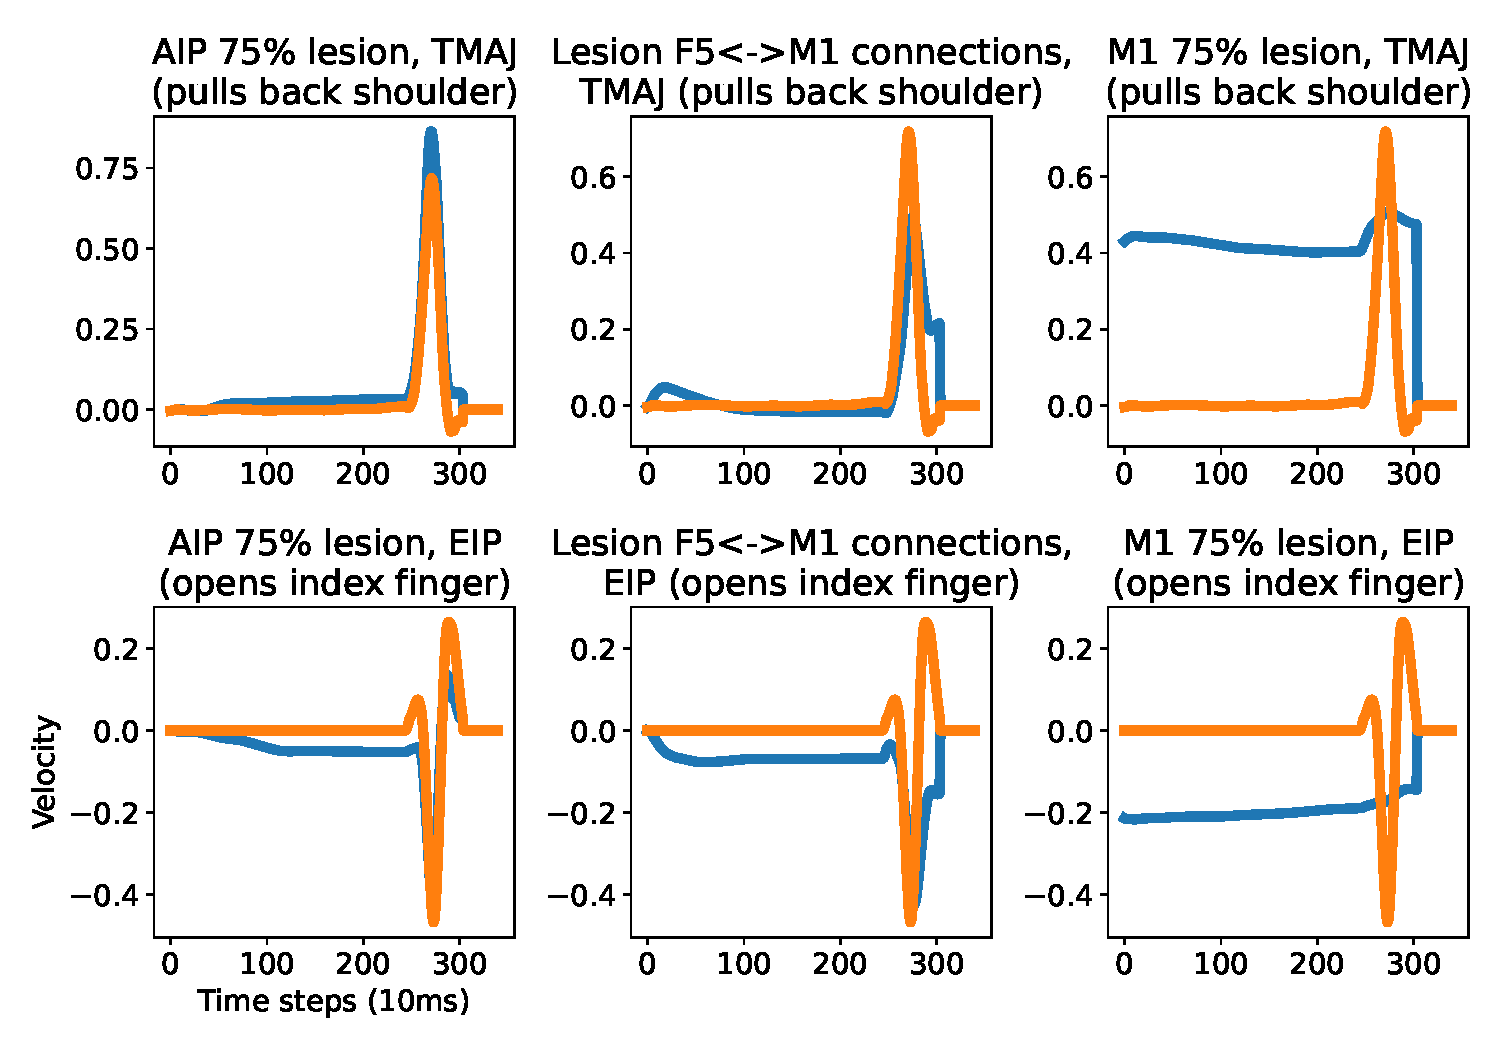
\includegraphics[width=\textwidth]{lesion_trajs.pdf}
	    \caption{Example muscle trajectories during a single trial, for one hand and shoulder muscle}
	\end{subfigure}
	\hfill
	\begin{subfigure}[c]{0.32\textwidth}
	    \centering
	    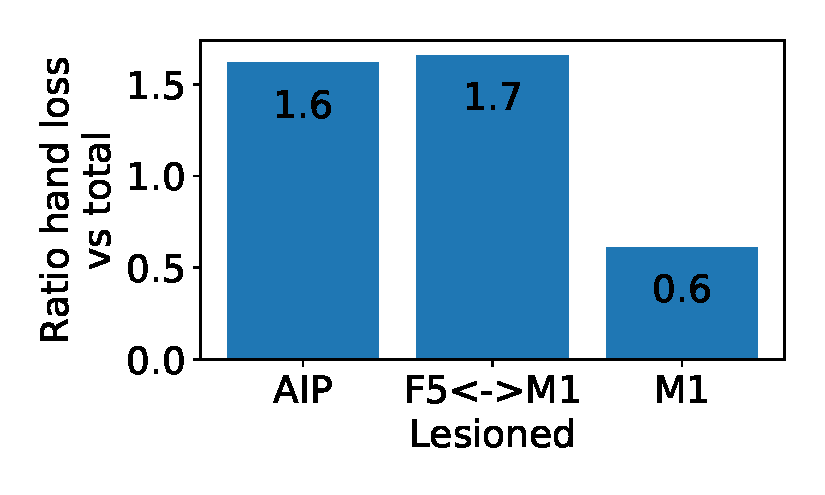
\includegraphics[width=\textwidth]{lesion_hand.pdf}
	    \caption{Proportion of loss attributable to hand muscles}
	\end{subfigure}
	\hfill
	\caption{Lesion designs which prevent forward propagation of object shape information
	         differentially impact hand pose. Loss here is an L2 distance
		 measured relative to the circuit's trajectories prior to the lesion.}
	\label{fig:lesion}
\end{figure}

The co-processor's task in our simulation will be to identify the appropriate information,
read from the mRNN's activations, for conditioning the stimulation. The co-processor seeks
to effectively bridge across the lesion, forward propagating the object shape information,
indirectly, through the use of stimulation.

In our experiments below, we demonstrate our co-processor design on three types of
simulated lesions:
\begin{itemize}
	\item \textbf{Output-based (AIP):} we force the output of some proportion of ``AIP''
	      neurons to zero, effectively removing them from the network. This results in a
	      loss of object shape information and, as we will see below, causes the co-processor
	      to be unable to differentiate objects.
	\item \textbf{Connection-based:} we prevent the forward and backward propagation of
	      information between the ``F5'' and ``M1'' modules, effectively representing a
	      severing of the connections between the two.
	\item \textbf{Output-based (M1):} we force the output of some proportion of ``M1''
	      neurons to zero, causing a more holisitic loss of movement.
\end{itemize}

\subsubsection{Simulated network exhibits long running dynamics}
Just as the co-processor must adapt to the lesion, it must also adapt to the dynamics of
the network it is stimulating. Natural neural networks as well as our simulated network
exhibit long running dynamics, which our CPN and EN must account for in their learning.
A perturbation of a network (i.e. due to stimulation) will cause changes in neuron
activations long after the stimulation is applied, sometimes far from the site of
stimulation. Our simulated grasping circuit exhibits the same behavior.

To illustrate this, suppose we applied a small, one-time, instantaneous perturbation
of the hidden state of 10 randomly chosen neurons in the output module at some point
in time during a trial. If we repeat that experiment many times, we can see what the
distribution of long- running effects tends to look like.

In Fig. \ref{fig:dynamics} we can see that even a single, one-time perturbation in
the network has effects dozens of time steps later. Our co-processor will need to
account for these, since stimulation is intended to cause perturbations in a network.
To successfully aid in grasping, the co-processor will need to account for these
dynamics. As we will show in the next subsection, the problem the co-processor faces
is in-fact even harder than this, due to a stimulation model that includes both
spatial and temporal smoothing.

\begin{figure}[h]
	\centering
	\begin{subfigure}[c]{0.48\textwidth}
	    \centering
	    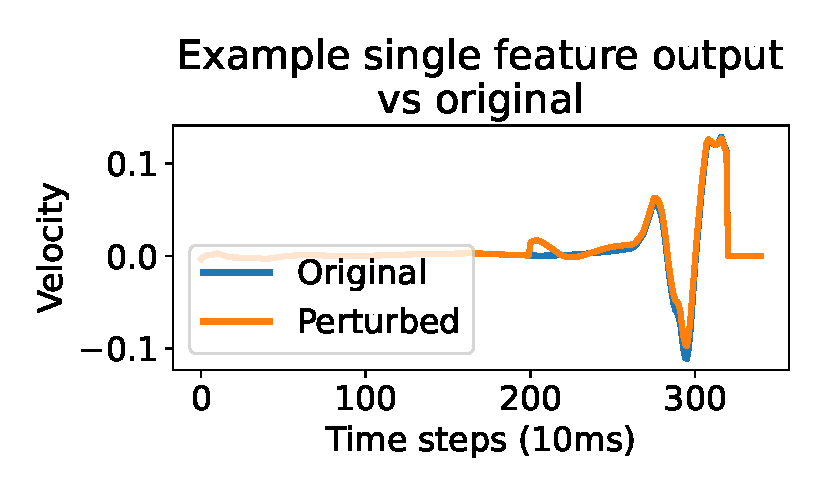
\includegraphics[width=\textwidth]{perturbe_single.pdf}
	    \caption{Example trial}
	\end{subfigure}
	\hfill
	\begin{subfigure}[c]{0.48\textwidth}
	    \centering
	    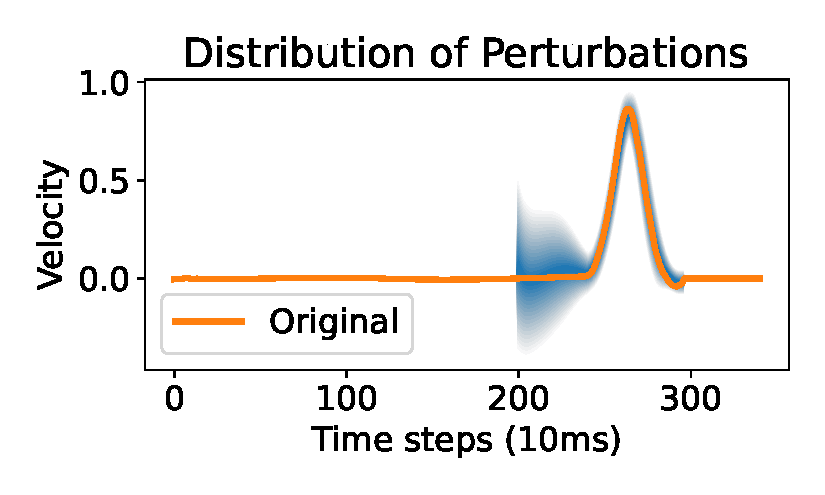
\includegraphics[width=\textwidth]{perturbe_dist.pdf}
	    \caption{Distribution of effects across n=1000 samples}
	\end{subfigure}
	\hfill
	\caption{Instantaneous perturbations of a random sample (n=10) of M1
	         neurons at time t=200 results in long-running effects on output.}
	\label{fig:dynamics}
\end{figure}

\subsubsection{Stimulation model}

\begin{figure}[h]
	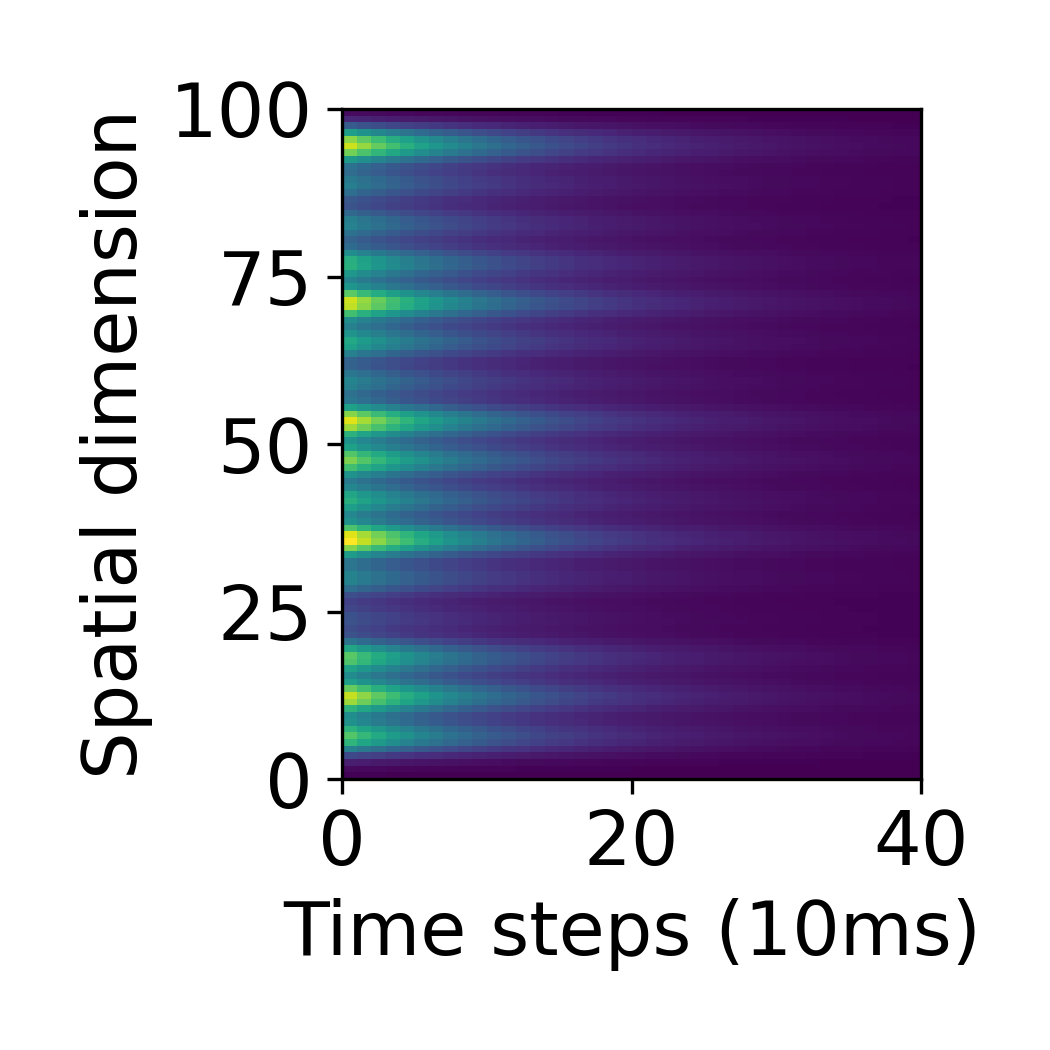
\includegraphics[width=0.45\textwidth]{stim_single.png}
	\caption{Spatial and temporal smoothing of a single 16 dimensional,
	         randomized $\theta$, onto 100 simulated neurons.
		 Color values indicate the magnitude of the value summed into
		 each neuron's hidden state in that time step. After $t=0$,
		 $\theta$ is the zero vector.}
	\centering
	\label{fig:stim_single}
\end{figure}

In order to inject another aspect of realism into our simulation, we subject
the co-processor to a stimulation model, rather than allowing it to directly
influence the hidden state of the simulated network's neurons. Our stimulation
model includes aspects of both spatial and temporal smoothing.

In our experiments, we stimulate only the output module, since this co-processor's
purpose is to improve external task performance, which it is able to do with
only stimulation of the output module of the network. It is conceivable that
a co-processor could stimulate other areas of the brain to improve task performance
downstream, or to probe the brain to better reveal the user's intent (i.e. object
shape), but we did not explore those possibilities in this paper.

The stimulation function $S$ receives as inputs the stimulation parameters $\theta$
provided by the CPN, which it accumulates in an internal memory. Each time step,
it outputs a modifier to the internal states of all neurons in the output module,
based on the current state of memory in the function object. That memory allows
the stimulation function to perform temporal smoothing. Specifically, we used a
simple exponential decay model where the function reads its current state of memory,
sums in the new parameters, and then decays each memory element towards $0.0$ at some
rate. Roughly speaking, this design intends to approximate the notion of dissipation: the
effect of stimulation is not instantaneous, but rather decays with time, as charge
dissipates into the surrounding area.

Likewise, the stimulation function maps the relatively low dimensional stimulation
parameter vector $\theta$ onto the M1 cells which it stimulates. In our experiments,
our stimulation parameters $\theta$ had 16 dimensions, which we found was
sufficient to allow significant improvement in task performance. The stimulation
function uses a simple Gaussian smoothing to map those parameters onto the simulated
M1 neurons. Each parameter represents, in a sense, an electrode located along a single
spatial dimension, whose stimulation affects the neurons in its vicinity more than
it affects others, according to each neuron's Mahalanobis distance from it. The neurons
are aligned along that dimension arbitrarily. We fix the width of the Gaussians
arbitrarily to $\sigma=1.75$. Note that we do not attempt to model the physical
layout of our simulated neurons, but simply want to disallow our co-processor
from having an unrealistically high degree of spatial resolution.

Thus, the governing equations of the stimulation become:

\begin{equation}
\alpha_{t} = \tau\alpha_{t-1} + \theta_{t}
\end{equation}
\begin{equation}
s_{t} = C(\alpha_{t})
\end{equation}

\begin{itemize}
	\item $\alpha$: the 16 dimensional internal activation, or memory
        of our stimulation
	\item $\tau$: our decay rate, which we set arbitrarily to $0.7$
	\item $C$: a precalculated $100 x 16$ matrix which provides our
	Gaussian smoothing
	\item $s_{t}$: the stimulation we apply to each neuron at the
	given time step.
\end{itemize}

The governing equations of the simulated network then become:

\begin{equation}
x_{t+1} = Jx_{t} + Iv_{t} + s_{t}
\end{equation}
\begin{equation}
a_{t} = tanh(x_{t})
\end{equation}
\begin{equation}
y_{t} = La_{t} + b
\end{equation}

\begin{itemize}
	\item $x$: the hidden state of each neuron
	\item $J$: the recurrence weight matrix
	\item $I$: the input response matrix
	\item $L$, $b$: the parameters of the linear readout
	\item $y$: the output of the network
\end{itemize}

See Fig. \ref{fig:stim_single} for a visual depiction of an example where
$\theta$ is non-zero at $t=0$, and zero for all other times, in order to see how
stimulation is applied across space and time. In Fig. \ref{fig:stim_and_obs},
we see stimulation applied during the simulation, in a real trial. In this case,
the trial is one where $50\%$ of M1 neurons are lesioned to have zero output.
Observations of the network's hidden state (explained in the next section) are taken
from the first two modules, and stimulation is applied to the last module. This fact
is intended to capture the difficulties with observing the same cortex that you are
stimulating, due to stimulation artifacts. The trial we show depicts stimulation
supplied by a highly trained co-processor, where task performance has been
largely restored. We explain this experiment in more detail below.

\begin{figure}[h]
	\centering
	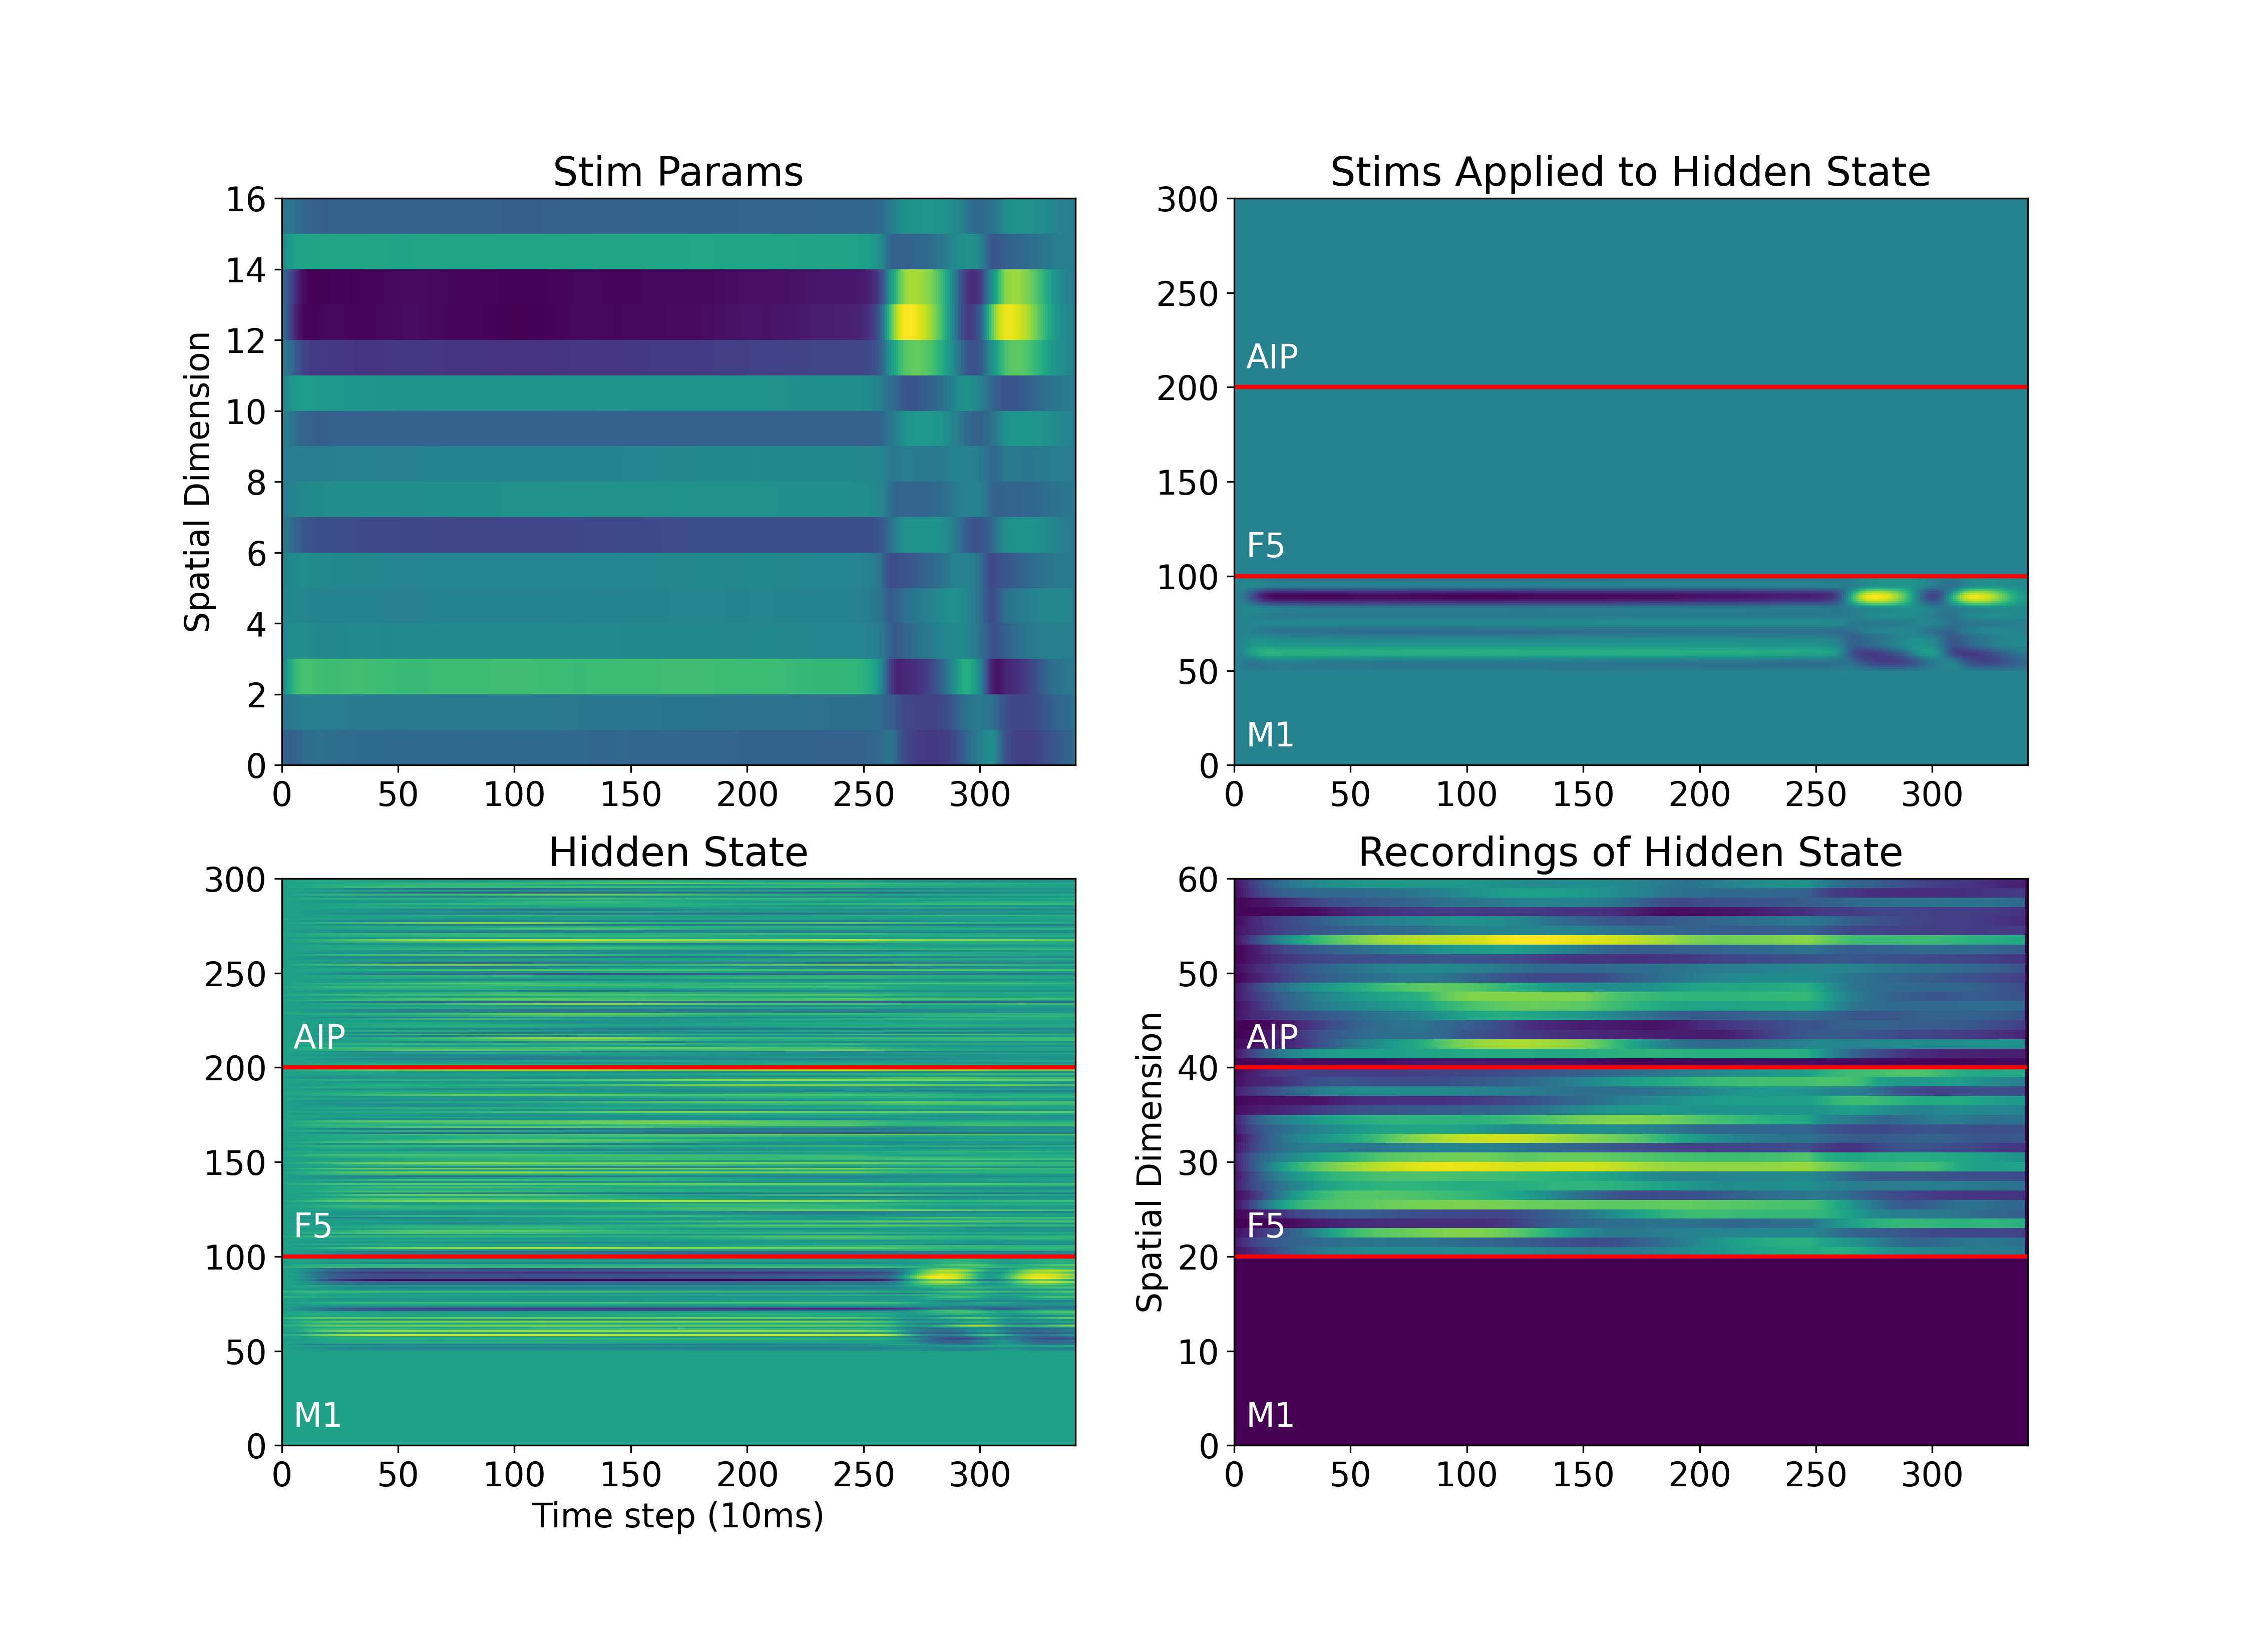
\includegraphics[width=\textwidth]{stim_and_obs.png}
	\caption{Example of stimulation and observation for a single trial. Here, M1
	has been lesioned 50\%, as seen in the zero (light blue) hidden states. We
	gather observations only from the AIP and F5 modules, as we explain in
	Section \ref{sec:experiments}. Stimulation is applied to M1, to drive the
	network output.}
	\label{fig:stim_and_obs}
\end{figure}

\subsubsection{Observation model}
Our observation model likewise relies on a notion of electrodes spread along
a single spatial dimension. As with stimulation, this is not intended to
capture true physical relationships between neurons and electrodes, but
rather to act as a dimensionality reduction that isn't designed to specifically
to favor task success, such as PCA. We treat the neurons of each module as
occupying their own space, with 20 electrodes arrayed along each.

We use a similar Gaussian-based approach as with stimulation, but in this
case our approach looks much like a Gaussian convolution, where the Gaussian
kernel is centered at each electrode position. Each `electrode' is read out
as a weighted average of all neurons in the given module, with weights being
provided by the Gaussian kernel. As above, refer to Fig. \ref{fig:stim_and_obs}
for a visual example.

\subsubsection{Brain co-adaptation}
To demonstrate the co-processor's ability to adapt to the non-stationarity
of the brain, we also change it throughout the co-processor's training.
Specifically, we simulate the brain's co-adaptation with the stimulation
to cooperatively solve the problem, as the stimulation is also changing
through the CPN's training.

We achieve this through a simple error backpropagation, using PyTorch's
implementation of the $Adam$ optimizer. With each trial, task loss is
calculated and backpropagated into the mRNN, allowing it to adapt to
its inputs, one of which is the stimulation being applied. The learning
rate for the optimizer is set arbitrarily to a relatively low rate of
$1e-7$.

\subsection{Training Algorithm}
In all experiments, training the co-processor requires a careful interleaving of
EN and CPN training epochs. EN training epochs concentrate on updating the EN,
based on observations of the effect of stimulation on the simulated network.
The loss function when training the EN is the MSE loss between the actual and
predicted output of the mRNN (i.e. muscle velocities). We then use the EN
to train the CPN during the CPN training epochs. During that time, we backpropagate
the MSE loss between the EN output, and target output, to the CPN. See Fig.
\ref{fig:training}.

TODO: explain EN training

\begin{figure}
	\centering
	\begin{subfigure}[c]{0.48\textwidth}
		\centering
		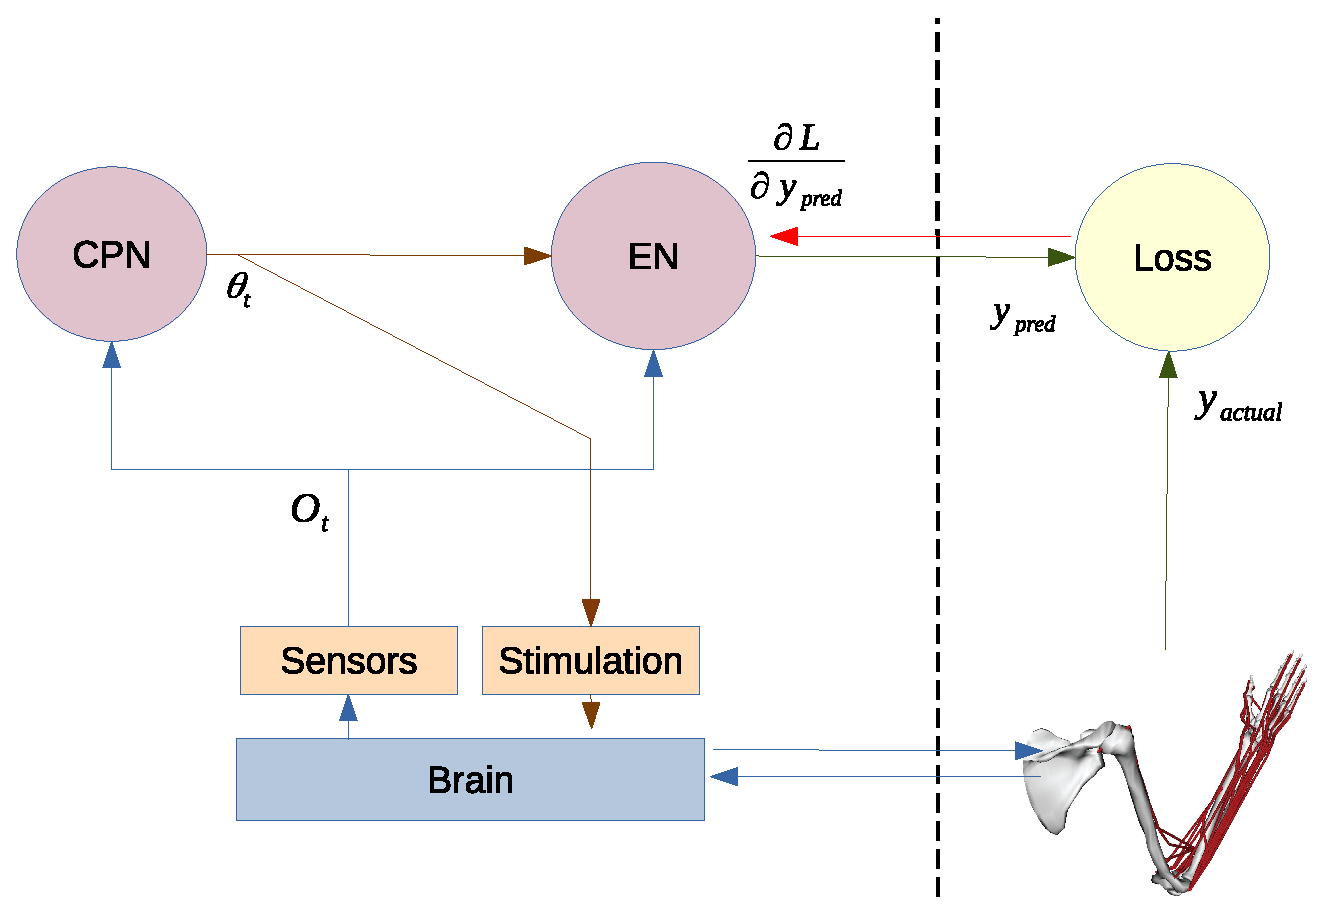
\includegraphics[width=\textwidth]{backprop_en.eps}
		\caption{EN training phase: backpropagate actual vs predicted}
	\end{subfigure}
	\hfill
	\begin{subfigure}[c]{0.48\textwidth}
		\centering
		\includegraphics[width=\textwidth]{backprop_cpn.eps}
		\caption{CPN training phase: backpropagate actual vs target MSE loss, via EN, to CPN. This effectively treats the EN output as the actual, and thus the EN must be trained first.}
	\end{subfigure}
	\hfill
\caption{Two Phase Training Regime}
\label{fig:training}
\end{figure}

Alternate training EN and CPN.
\begin{itemize}
	\item Train an EN
		\begin{itemize}
			\item Training the EN until predictive power reaches a threshold, based on current task performance
			\item Training regime based on most recent CPN, similar CPNS (noise added to params), and white noise stimulation
			\item Single batch of data from applying current CPN set and white noise to the brain, EN fit to ``offline'' it over maining epochs
			\item Predictive power alone is not sufficient for use in training the CPN: we need to form the batch as above, otherwise training is unstable.
			\item White noise and noised params
			\item ** Learning instability
			\item ** Predictive power isn't enough
			\item ** Illustrate this
		\end{itemize}
	\item Train the CPN
		\begin{itemize}
			\item Backprop through the EN, effectively using the EN's prediction as ground truth
		\end{itemize}

	\item Data recycling/reuse
\end{itemize}

\begin{figure}[h]
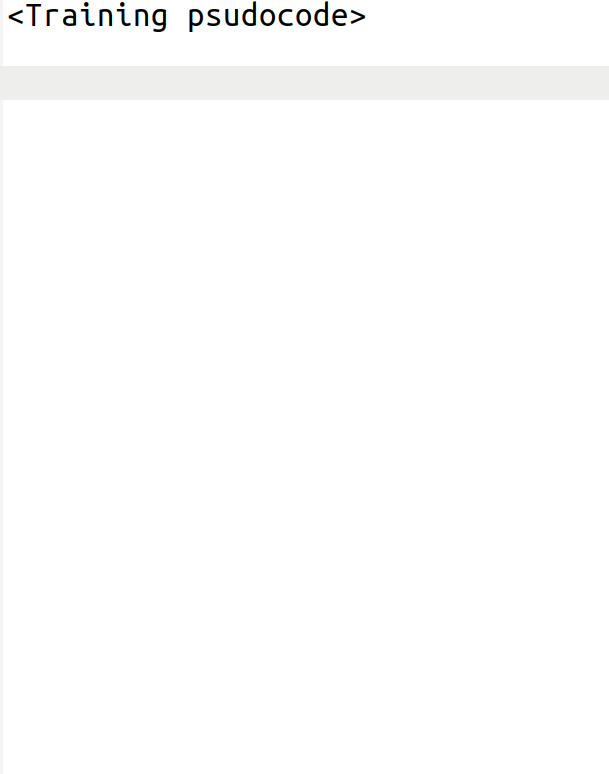
\includegraphics[width=0.5\textwidth]{pseudocode.png}
\caption{Pseudocode of the Training Method}
\centering
\label{fig:pseudocode}
\end{figure}

\subsection{Experiments}
\label{sec:experiments}

Using the simulation described above, we perform three experiments to
demonstrate the co-processor's ability to learn:
\begin{itemize}
	\item 50\% AIP loss
	\item 100\% connectivity lesion between the F5 and M1 modules
	\item 50\% M1 loss
\end{itemize}

Additionally, we perform each of the ...

Summary of tunables:
\begin{itemize}
	\item Learning rate schedules
	\item Activation functions
	\item Obs function dimensionality
	\item Stim dimensionality
	\item Dimensionality of EN, CPN
\end{itemize}

\begin{figure}
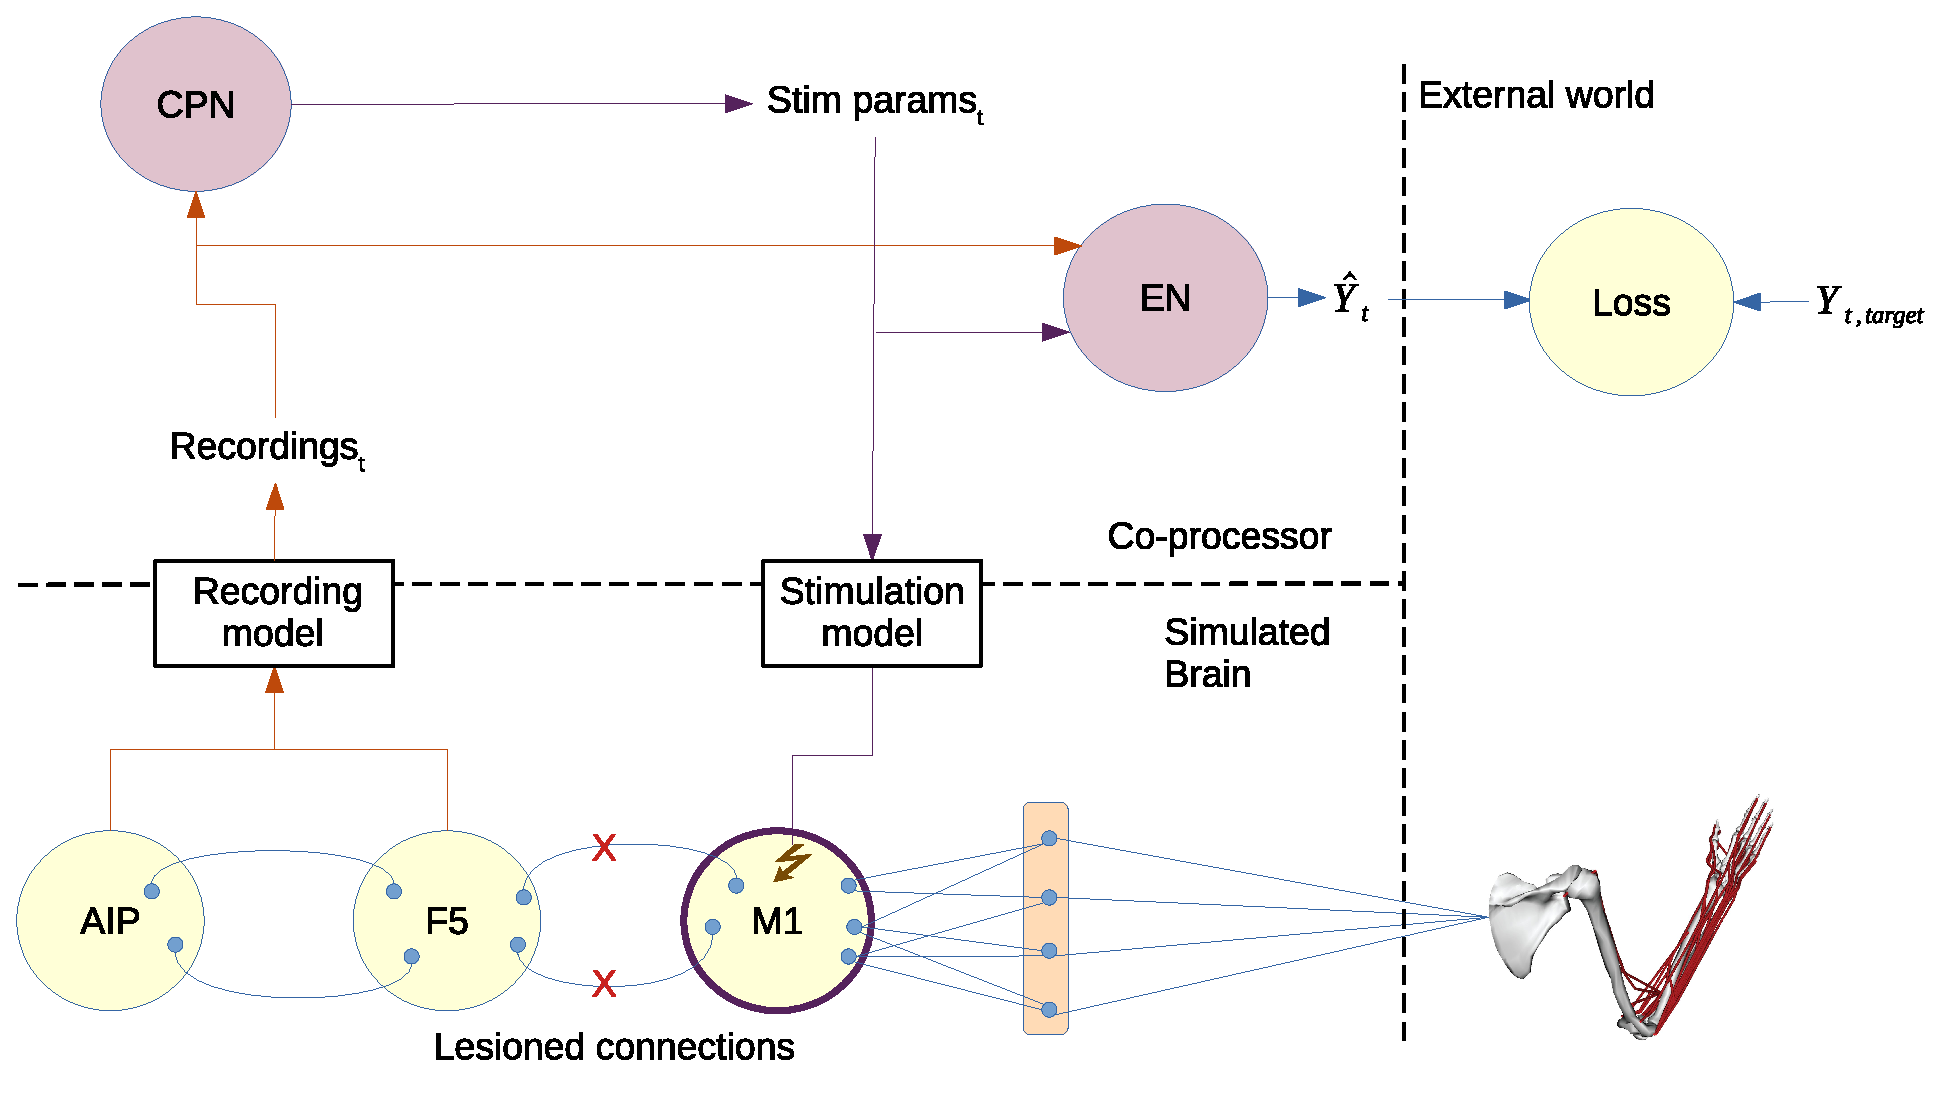
\includegraphics[width=\textwidth]{cpn_michaels_arch_labeled.eps}
\caption{Experiment architecture overview}
\centering
\label{fig:exp_overview}
\end{figure}

\section{Results}

\begin{figure}[h]
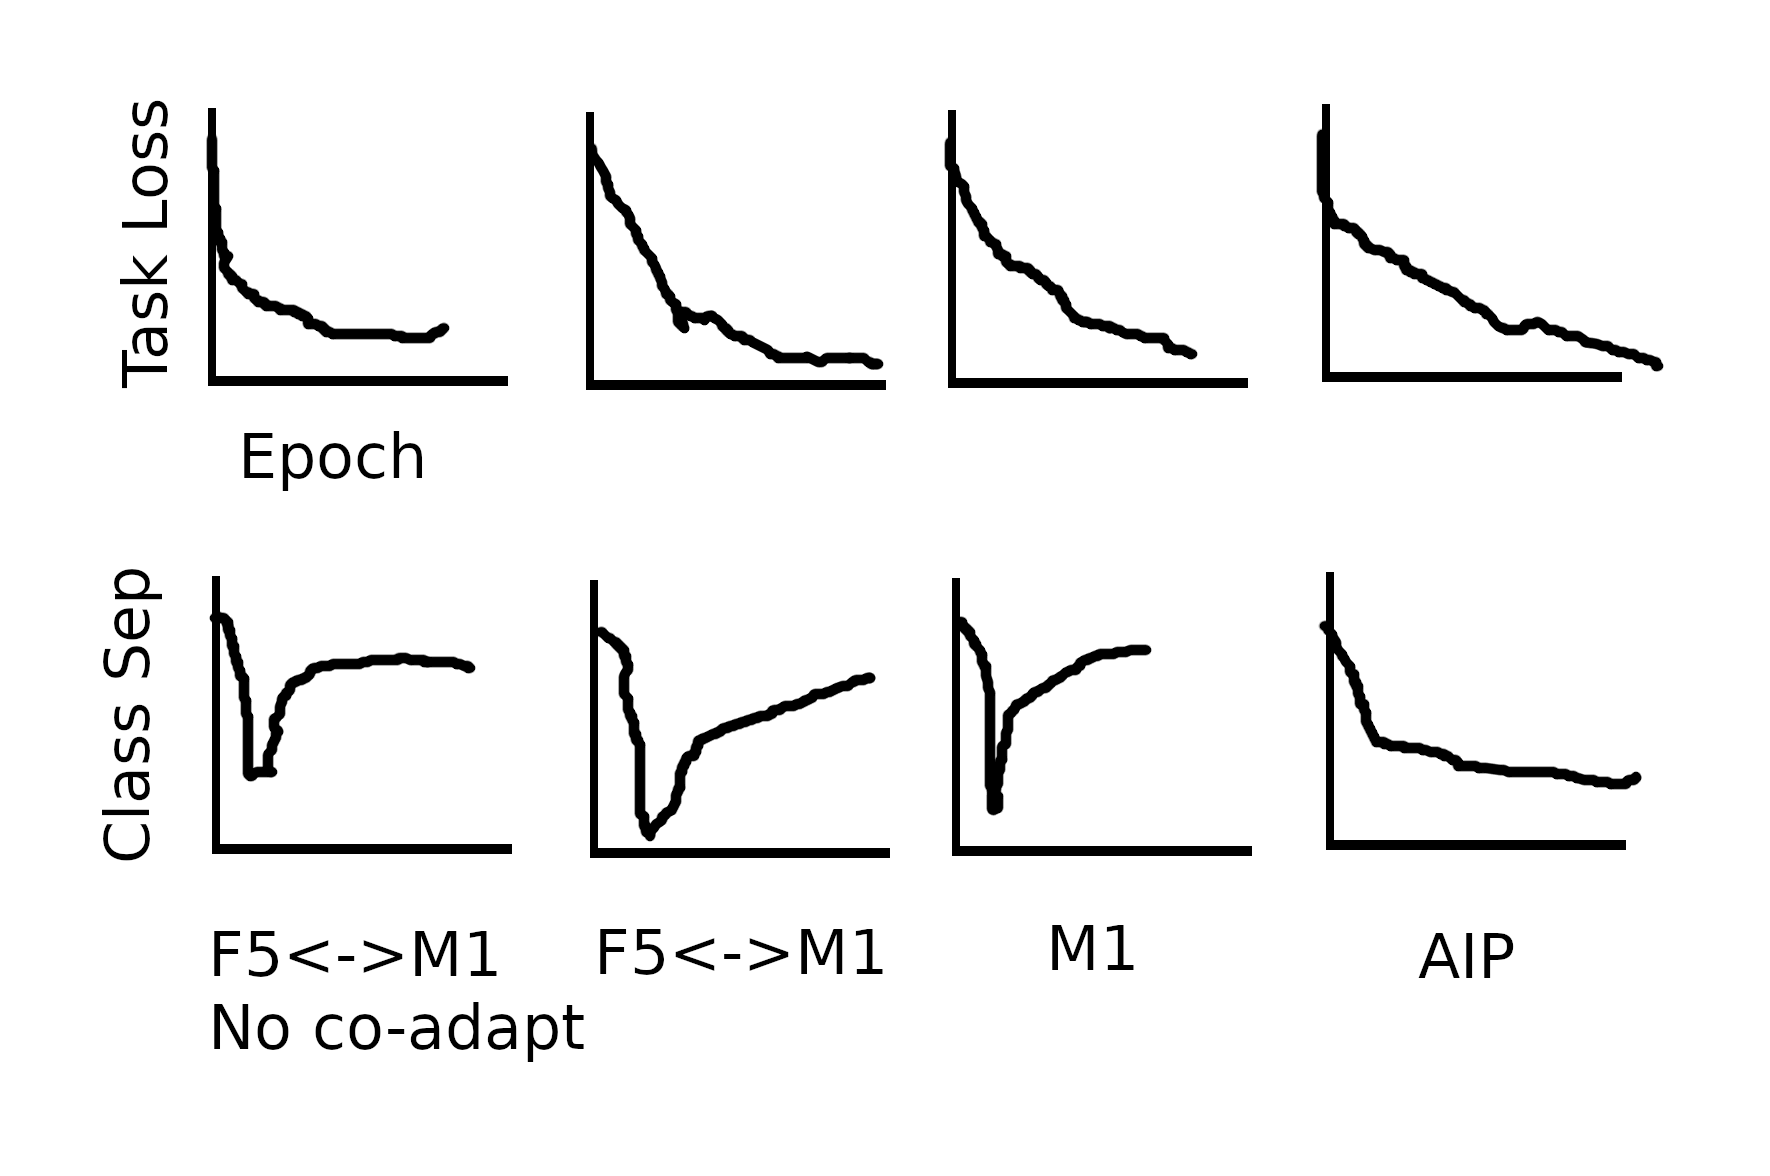
\includegraphics[width=\textwidth]{results_standin.png}
\caption{Loss and class separation vs training epoch}
\centering
\label{fig:results}
\end{figure}

\begin{itemize}
	\item Task performance improves drastically.
		\begin{itemize}
			\item Fig: normalized task loss vs CPN training epoch
			\item Fig: normalized task loss vs training epoch
			\item Fig: normalized task loss vs training epoch
			\item Split by experiment
		\end{itemize}
	\item Fine tuning takes a long time
	\item Object classes separate. Fig: sep vs experiment vs epoch
	\item Can co-adapt with the brain, as it changes
	\item Training efficiency analysis. Show num epochs with and without recycling.
\end{itemize}

\section{Discussion and Conclusion}
\begin{itemize}
	\item Training efficiency
	\item Spectrum from simple low dimensional stimulation vectors today to higher dimensional future
	\item Toward in vivo application
\end{itemize}

\section{Acknowledgements}
Ganguly, Priya, Anca, Justin, Luciano

\section{Ethical Statement}
asdf

\section{References}
\bibliographystyle{iopart-num}
\bibliography{refs}
\end{document}

